\section{M21}\label{sec:m21}

\subsection{Instalação e uso}

\subsubsection*{Pelo terminal}
Considerando que o sistema operacional já possui o \emph{git}\footnote{https://en.wikipedia.com/git}, podem ser dados os seguintes comando em um terminal.

\begin{minted}[linenos,frame=leftline,fontsize=\footnotesize]{python}
guilherme@R410-L-BP12P1 > git clone https://www.github.com/jahpd/m21.git
guilherme@R410-L-BP12P1 > cd m21
guilherme@R410-L-BP12P1 > chmod u+x ./m21
\end{minted}

\subsubsection*{Opções}

Ao executar o comando $help$ é obtida uma página de ajuda.

\begin{minted}[linenos,frame=leftline,fontsize=\scriptsize]{python}
guilherme@R410-L-BP12P1 > ./m21 --help
Usage: m21 [OPTIONS, [ARGS]]

For computer assisted musicology and composition

Options:
  --version             show program's version number and exit
  -h, --help            show this help message and exit
  -s, --search-only     Search in corpus for words in --composer and or
                        --index arguments. Ex.: --composer bach --index bwv1x
  -c COMPOSER, --composer=COMPOSER
                        write report with specific corpora. CAUTION: you must
                        use this according http://web.mit.edu/music21/doc/syst
                        emReference/referenceCorpus.html#referencecorpus
  -i INDEX, --index=INDEX
                        Search in corpus specific index of corpora; you must
                        use this with -c option, according available corpora
                        in  http://web.mit.edu/music21/doc/systemReference/ref
                        erenceCorpus.html#referencecorpus
  -C, --CAC             Or simple "Computer Assisted Composition". With this
                        option you will "glitch" a specific piece, as
                        instance, with --composer/--index options, --xml
                        option or --tiny-notation option. Adding --fragmentize
                        option with a value (ex: --fragmentize 4, max 6), you
                        will apply a "fragmentation" on input. You can add
                        --no-scramble-notes, --no-scramble-octaves and
                        arguments.
  -n, --no-scramble-notes
                        with this option, the program will not apply a
                        scramble on list of extracted notes, before create
                        chords
  -N, --no-scramble-octaves
                        With this option, the program will not apply a
                        scramble on list of extracted octaves, before create
                        chords
  -g GLITCH, --glitch=GLITCH
                        Apply a'glitch' on extracted notes and octaves; the
                        given argument is the maximum of a random operation.
                        This operation can be a choice of a 6 values: (0) The
                        generated chord will be arranged in closed position;
                        (1) the generated chord will be arranged in semi-
                        closed position; (2) the generated chord will be
                        arranged in super open position; (3) one note will be
                        separated from chord, like an one grace note; (4) two
                        notes will be separated from chord (if this chord have
                        at least, two notes); (5) apply bordadure [? translate
                        ?], and then a chord
  -m MEASURES, --measures=MEASURES
                        Select measures from a stream (corpus, xml or
                        tinynotation)
  -R, --reducte         Reducte some stream to piano staff
  -A TONAL_HARMONIC_ANALYSIS, --tonal-harmonic-analysis=TONAL_HARMONIC_ANALYSIS
                        Analyse some stream in tonal way, given some key
  -S, --show            show stream in some editor (musescore default)
  -x XML, --xml=XML     parse a musicXml file; can be a local one or http url
  -t TINYNOTATION, --tinynotation=TINYNOTATION
                        parse a tiny-notation (ex: --tiny-notation "2/16 E4 r
                        f# g=lastG trip{b-8 a g} c".
  -T TITLE, --title=TITLE
                        used to give a title. (ex: --title "My improvised
                        music"
  -a AUTHOR, --author=AUTHOR
                        used to give a author. (ex: --author "J.S. Bach"
  -r TRANSPOSE, --transpose=TRANSPOSE
                        transpose stream notes by semitones (ex.: --transpose
                        4 will transpose to a ascendent major third and
                        --transpose -4 will transpose to a descendent major
                        third
  -I, --invert          invert stream intervals by semitones. No need
                        arguments
  -L LYTEXIFY, --lytexify=LYTEXIFY
                        Create a .lytex file from a .ly file, and compiles it
                        to a .tex file. Used only in the context of
                        documentation of this software
  --plot-stream         analysis graph with PlotStream class
  --plot-histogram-pitch-space
                        analysis graph with PlotHistogramPitchSpace class
  --plot-histogram-pitch-class
                        analysis graph with PlotHistogramPitchClass class
  --plot-histogram-quarter-length
                        analysis graph with PlotHistogramQuarterLength class
  --plot-scatter-pitch-space-quarter-length
                        analysis graph with PlotScatterPitchSpaceQuarterLength
                        class
  --plot-scatter-pitch-class-quarter-length
                        analysis graph with PlotScatterPitchClassQuarterLength
                        class
  --plot-scatter-pitch-class-offset
                        analysis graph with PlotScatterPitchClassOffset class
  --plot-scatter-pitch-space-dynamic-symbol
                        analysis graph with PlotScatterPitchSpaceDynamicSymbol
                        class
  --plot-horizontal-bar-pitch-space-offset
                        analysis graph with PlotHorizontalBarPitchSpaceOffset
                        class
  --plot-horizontal-bar-pitch-class-offset
                        analysis graph with PlotHorizontalBarPitchClassOffset
                        class
  --plot-scatter-weighted-pitch-space-quarter-length
                        analysis graph with
                        PlotScatterWeightedPitchSpaceQuarterLength class
  --plot-scatter-weighted-pitch-class-quarter-length
                        analysis graph with
                        PlotScatterWeightedPitchClassQuarterLength class
  --plot-scatter-weighted-pitch-space-dynamic-symbol
                        analysis graph with
                        PlotScatterWeightedPitchSpaceDynamicSymbol class
  --plot3-d-bars-pitch-space-quarter-length
                        analysis graph with Plot3DBarsPitchSpaceQuarterLength
                        class
  --plot-windowed-krumhansl-schmuckler
                        analysis graph with PlotWindowedKrumhanslSchmuckler
                        class
  --plot-windowed-krumhansl-kesslerm
                        analysis graph with PlotWindowedKrumhanslKesslerm
                        class
  --plot-windowed-aarden-essen
                        analysis graph with PlotWindowedAardenEssen class
  --plot-windowed-simple-weights
                        analysis graph with PlotWindowedSimpleWeights class
  --plot-windowed-bellman-budge
                        analysis graph with PlotWindowedBellmanBudge class
  --plot-windowed-temperley-kostka-payne
                        analysis graph with PlotWindowedTemperleyKostkaPayne
                        class
  --plot-windowed-ambitus
                        analysis graph with PlotWindowedAmbitus class
  --plot-dolan          analysis graph with PlotDolan class
\end{minted}

\subsubsection*{Alguns usos básicos}

Os comandos podem ter sua forma longa e curta; por exemplo \verb|--composer| pode ser abreviado para \verb|-c|. Abaixo listamos alguns dos mais usados durante o trabalho

\subsubsection*{Procurar por compositores ou obras  no \emph{corpus}}:
\begin{minted}[linenos,frame=leftline,fontsize=\footnotesize]{python}
./m21 --search-only --composer bach
./m21 -s -c bach -i bwv1
./m21 --search-only --index bwv1
./m21 -s -i bwv1
\end{minted}

\subsubsection*{Mostrar em um \emph{software} de editoração musical uma obra do \emph{corpus}.}

De acordo com a documentação oficial, um \emph{software} externo pode ser usado para abrir aquivos formatados em \emph{musicXml}. Como é um formato padrão, diferentes editores de partitura podem ser usados. Entre eles Finale e Sibelius. Neste artigo utilizamos o \cite{musescore_2015}. Para alterar qual deles será usado, é necessário modificar a variável \verb|musicxmlPath| no arquivo \verb|~/.music21.rc| (em sistemas Unix), criado durante a instalação.

\begin{minted}[linenos,frame=leftline,fontsize=\footnotesize]{python}
./m21 --show --composer bach --index bwv1
./m21 -S -c bach -i bwv1
\end{minted}

\subsubsection*{Mostrar no Musescore um arquivo do tipo musicxml.}

\begin{minted}[linenos,frame=leftline,fontsize=\footnotesize]{python}
./m21 --show --xml bwv1.xml
./m21 -S -x bwv1.xml
\end{minted}

\subsubsection*{Mostrar no Musescore uma idéia musical improvisada.}

É possível escrever rapidamente uma idéia musical. Um pequeno exemplo de codificação foi realizado abaixo com um motivo da primeira invenção de Bach.

\begin{minted}[linenos,frame=leftline,fontsize=\footnotesize]{python}
./m21 -show --tinynotation "2/4 r16 c d e f d e c g8 c' b c' d'"
./m21 -S -t "2/4 r16 c d e f d e c g8 c' b c' d'"
\end{minted}

\begin{figure}[h]
  \centering
  {%
\parindent 0pt
\noindent
\ifx\preLilyPondExample \undefined
\else
  \expandafter\preLilyPondExample
\fi
\def\lilypondbook{}%

\includegraphics{../examples/tinynotation/42/lily-08b23daa-1}%
\ifx\betweenLilyPondSystem \undefined
  \linebreak
\else
  \expandafter\betweenLilyPondSystem{1}%
\fi

\includegraphics{../examples/tinynotation/42/lily-08b23daa-2}%
% eof

\ifx\postLilyPondExample \undefined
\else
  \expandafter\postLilyPondExample
\fi
}

  \caption{Motivo principal da invenção em dó maior J.S. Bach, BWV X, escrito rapidamente n terminal. Metadados necessitam de correções \textbf{Fonte}: autor}
    \label{fig:tinynotation}
\end{figure}

\subsubsection*{Mostrar no Musescore um recorte de uma obra no \emph{corpus}.}

Apresentar um fragmento de uma peça. Abaixo recortei os cinco primeiros compassos do BWV1, como na figura \ref{fig:bwv_frag}:

\begin{minted}[linenos,frame=leftline,fontsize=\footnotesize]{python}
./m21 --show --composer bach --index bwv1 --measures 0 4
./m21 -S -c bach -i bwv1 -m 0 4
\end{minted}

\begin{figure}[h]
  \centering
  {%
\parindent 0pt
\noindent
\ifx\preLilyPondExample \undefined
\else
  \expandafter\preLilyPondExample
\fi
\def\lilypondbook{}%

\includegraphics{../analysis/bwv1/2a/lily-0aa3d7a2-1}%
\ifx\betweenLilyPondSystem \undefined
  \linebreak
\else
  \expandafter\betweenLilyPondSystem{1}%
\fi

\includegraphics{../analysis/bwv1/2a/lily-0aa3d7a2-2}%
\ifx\betweenLilyPondSystem \undefined
  \linebreak
\else
  \expandafter\betweenLilyPondSystem{2}%
\fi

\includegraphics{../analysis/bwv1/2a/lily-0aa3d7a2-3}%
% eof

\ifx\postLilyPondExample \undefined
\else
  \expandafter\postLilyPondExample
\fi
}

  \caption{Extração dos cinco primeiros compassos (\emph{measures}) do BWV1.6, utilizando o comando \emph{./m21 -c bach -i bwv1 -m 0 4}}
    \label{fig:bwv_frag}
\end{figure}

\subsubsection*{Analisar uma peça tonal} 

Por exemplo, os cinco primeiros compassos anteriores (quatro compassos e anacruse) podem ser analisados em qualquer tom. Considerando que o grau I é Fá, indicamos na linha de comando a representação alfabética, ou a letra \textbf{F} será apresentado o resultado como na figura \ref{fig:bwv_anal}. Qualquer outra nota utilizada para análise irá gerar um ``processo proporcional'', mas incorreto do ponto de vista da tradição didática musical. Certamente informações podem aparecer incorretamente e outras são redundantes. Tais critérios, ainda a serem discutidos e programados, serão importantes para desenvolvimentos futuros.

\begin{minted}[linenos,frame=leftline,fontsize=\footnotesize]{python}
./m21 --show --composer bach --index bwv1 --tonal-harmonic-analysis F
./m21 -S -c bach -i bwv1 -m 0 9 -A F
\end{minted}
 
\begin{figure}
  \centering
  {%
\parindent 0pt
\noindent
\ifx\preLilyPondExample \undefined
\else
  \expandafter\preLilyPondExample
\fi
\def\lilypondbook{}%

\includegraphics{../analysis/bwv1/aa/lily-baff07b9-1}%
\ifx\betweenLilyPondSystem \undefined
  \linebreak
\else
  \expandafter\betweenLilyPondSystem{1}%
\fi

\includegraphics{../analysis/bwv1/aa/lily-baff07b9-2}%
\ifx\betweenLilyPondSystem \undefined
  \linebreak
\else
  \expandafter\betweenLilyPondSystem{2}%
\fi

\includegraphics{../analysis/bwv1/aa/lily-baff07b9-3}%
\ifx\betweenLilyPondSystem \undefined
  \linebreak
\else
  \expandafter\betweenLilyPondSystem{3}%
\fi

\includegraphics{../analysis/bwv1/aa/lily-baff07b9-4}%
\ifx\betweenLilyPondSystem \undefined
  \linebreak
\else
  \expandafter\betweenLilyPondSystem{4}%
\fi

\includegraphics{../analysis/bwv1/aa/lily-baff07b9-5}%
% eof

\ifx\postLilyPondExample \undefined
\else
  \expandafter\postLilyPondExample
\fi
}

  \caption{Análise harmônica automática dos cinco primeiros compassos, na tonalidade de Fá Maior  }
    \label{fig:bwv_anal}
\end{figure}

\subsubsection*{Plotar histogramas.}

Comandos de plotagem não possuem versões minificadas. Muitas delas possuem problemas de compatibilidade com o fragmento a ser analisado e a opção fornecida. Um exemplo de análise da classe de altura mais usada em um fragmento, ou peça inteira, é demonstrado na figura \ref{fig:pitch-class-bwv1-histogram}.

\begin{minted}[linenos,frame=leftline,fontsize=\footnotesize]{python}
./m21 --show --composer bach --index bwv1 --plot-histogram-pitch-space
./m21 -S -c bach -i bwv1 --plot-histogram-pitch-space
\end{minted}

\begin{figure}[h]
  \centering
  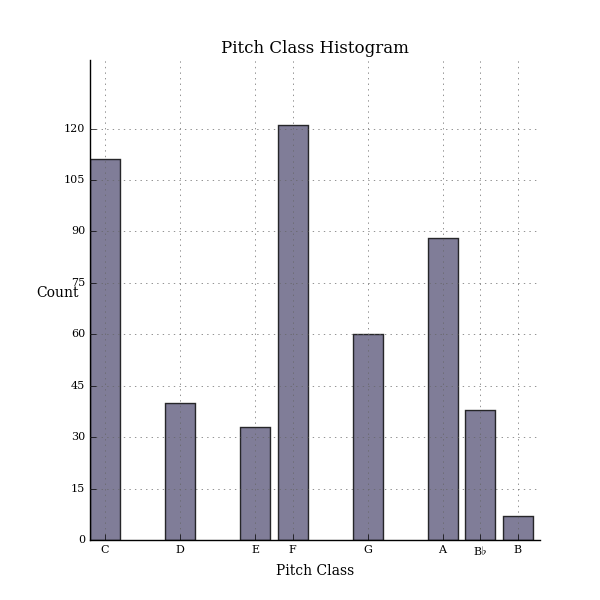
\includegraphics[scale=0.71]{../analysis/bwv1/pitch-class.png}
  \caption{Histograma de \emph{pitch-class} do BWV1.6. \textbf{Fonte}: autor utilizando Music21.}
    \label{fig:pitch-class-bwv1-histogram}
\end{figure}